\documentclass[11pt,oneside,notitlepage,a4paper,wide]{mwart}
\usepackage[utf8]{inputenc}
\usepackage{polski}

\usepackage{enumitem}
	\setlist{nolistsep}
	\renewcommand{\labelitemi}{$\bullet$}
	% \renewcommand{\labelitemii}{$\bullet$}
	
\usepackage{makeidx}
\usepackage{graphicx}
\usepackage{setspace}

\onehalfspacing
\setlength{\parindent}{0 cm} % Rozmiar wcięcia akapitów.

\usepackage[final]{pdfpages}

\usepackage[]{hyperref}
\usepackage{xcolor}
	\definecolor{orangelink}{rgb}{0.7,0.18,0.1}

	\hypersetup{ 
		pdftitle={Alleluia Pasquale – Dominica Paschæ in Resurrectione Domini – Ad Vigiliam Paschalem in Nocte Santa},
			pdfdisplaydoctitle=true,
		pdfauthor={pitrk, JanekR_Prorok},
  		pdfsubject={Source: https://github.com/JanekRProrok/Triduum_Sacrum},
    	pdfcreator={Texmaker, MiKTeX},
		% pdfproducer={},
		% pdfinfo={},
		% pdfkeywords={},
		bookmarks=true,
		bookmarksnumbered=true,
		bookmarksopen=true,
			bookmarksopenlevel=1,
		pdfpagelabels=true,
		pdfpagemode=UseOutlines,
		unicode=true,
		pdftoolbar=true,
		pdfmenubar=true,
		pdffitwindow=false,
		pdfstartview=Fit,
		pdfnewwindow=true,
		colorlinks=true,
		linkcolor=orangelink,
		citecolor=orangelink,
		filecolor=orangelink,
		urlcolor=orangelink,
		pdfpagelayout=OneColumn,
		% pdfstartpage=1,
		% pdfnumcopies=2, % Domyślna liczba drukowanych kopii
	}
 
%%%%%%%%%%%%%%%%%%%%%%%%%%%%%%%%%%%%%%%%%%%%%%%%%%%%%%%%%%%%%%%%%%%%%%%%%%%%%%%%%%%%%%%%%%%%%%%%%%%%%%%%%%%%%%%%%%%%%%%%%%%%%%%%%%%%%%%%%%
%%%%%%%%%%%%%%%%%%%%%%%%%%%%%%%%%%%%%%%%%%%%%%%%%%%%%%%%%%%% TREŚĆ DOKUMENTU %%%%%%%%%%%%%%%%%%%%%%%%%%%%%%%%%%%%%%%%%%%%%%%%%%%%%%%%%%%%%
%%%%%%%%%%%%%%%%%%%%%%%%%%%%%%%%%%%%%%%%%%%%%%%%%%%%%%%%%%%%%%%%%%%%%%%%%%%%%%%%%%%%%%%%%%%%%%%%%%%%%%%%%%%%%%%%%%%%%%%%%%%%%%%%%%%%%%%%%%

\begin{document}
% \sloppy % - Wymuszenie nieprofesjonalnego trzymania się w marginesach jak w MS Word (kosztem dziwnie rozciągniętych odstępów -
	% LaTeX uważa, że lepiej wyjątkowo wyjść ze zbyt długim wyrazem kawałek na margines niż umieszczać między wyrazami
	% kilkucentymetrowe odstępy).

% pdftitle={Dominica Paschæ in Resurrectione Domini - Ad Vigiliam Paschalem in Nocte Santa}
	{\centering\LARGE{\textbf{Dominica Paschæ in Resurrectione Domini\\Ad Vigiliam Paschalem in Nocte Santa}}\\\smallskip\large{Niedziela Zmartwychwstania Pańskiego\\Wigilia Paschalna w Wielką Noc}\par\vspace{5 mm}}

Po odczytaniu Epistoły wszyscy wstają, a kapłan uroczyście intonuje \emph{Alleluia}, które wszyscy powtarzają. Jeśli to konieczne, sam psalmista intonuje \emph{Alleluia}.

	\begin{figure}[h] \centering 
		\includegraphics[width=\textwidth]{Alleluia_choral.png}
		
		\medskip
		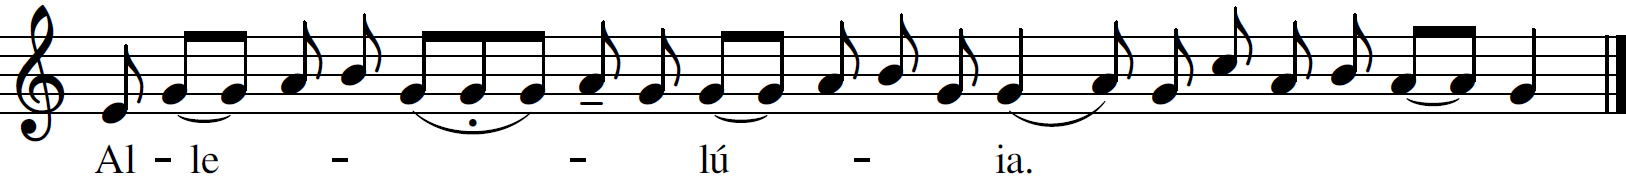
\includegraphics[width=\textwidth]{Alleluia_nuty.png}
	\end{figure}

Aklamację powtarza się trzykrotnie, za każdym razem od kolejnego, dwa półtony wyższego, dźwięku. Następnie psalmista lub kantor śpiewa psalm, a lud powtarza refren \emph{Alleluia}.

Na drugiej stronie podano przykładowe transpozycje aklamacji.\bigskip

Przykładowe wykonania:
	\begin{enumerate}[label=\alph*),leftmargin=1.25 cm]
		\item Watykan 2011 -- \href{https://youtu.be/4DvRrrdOfbo}{https://youtu.be/4DvRrrdOfbo}
		\item Watykan 2013 -- \href{https://youtu.be/k89SA3lBdKI}{https://youtu.be/k89SA3lBdKI}
		\item Frombork 2015 -- \href{https://youtu.be/kpDhlek1h0w}{https://youtu.be/kpDhlek1h0w}
		\item Pogórze 2018 -- \href{https://youtu.be/MJ4hgMCgcRI}{https://youtu.be/MJ4hgMCgcRI}	
	\end{enumerate}
\newpage 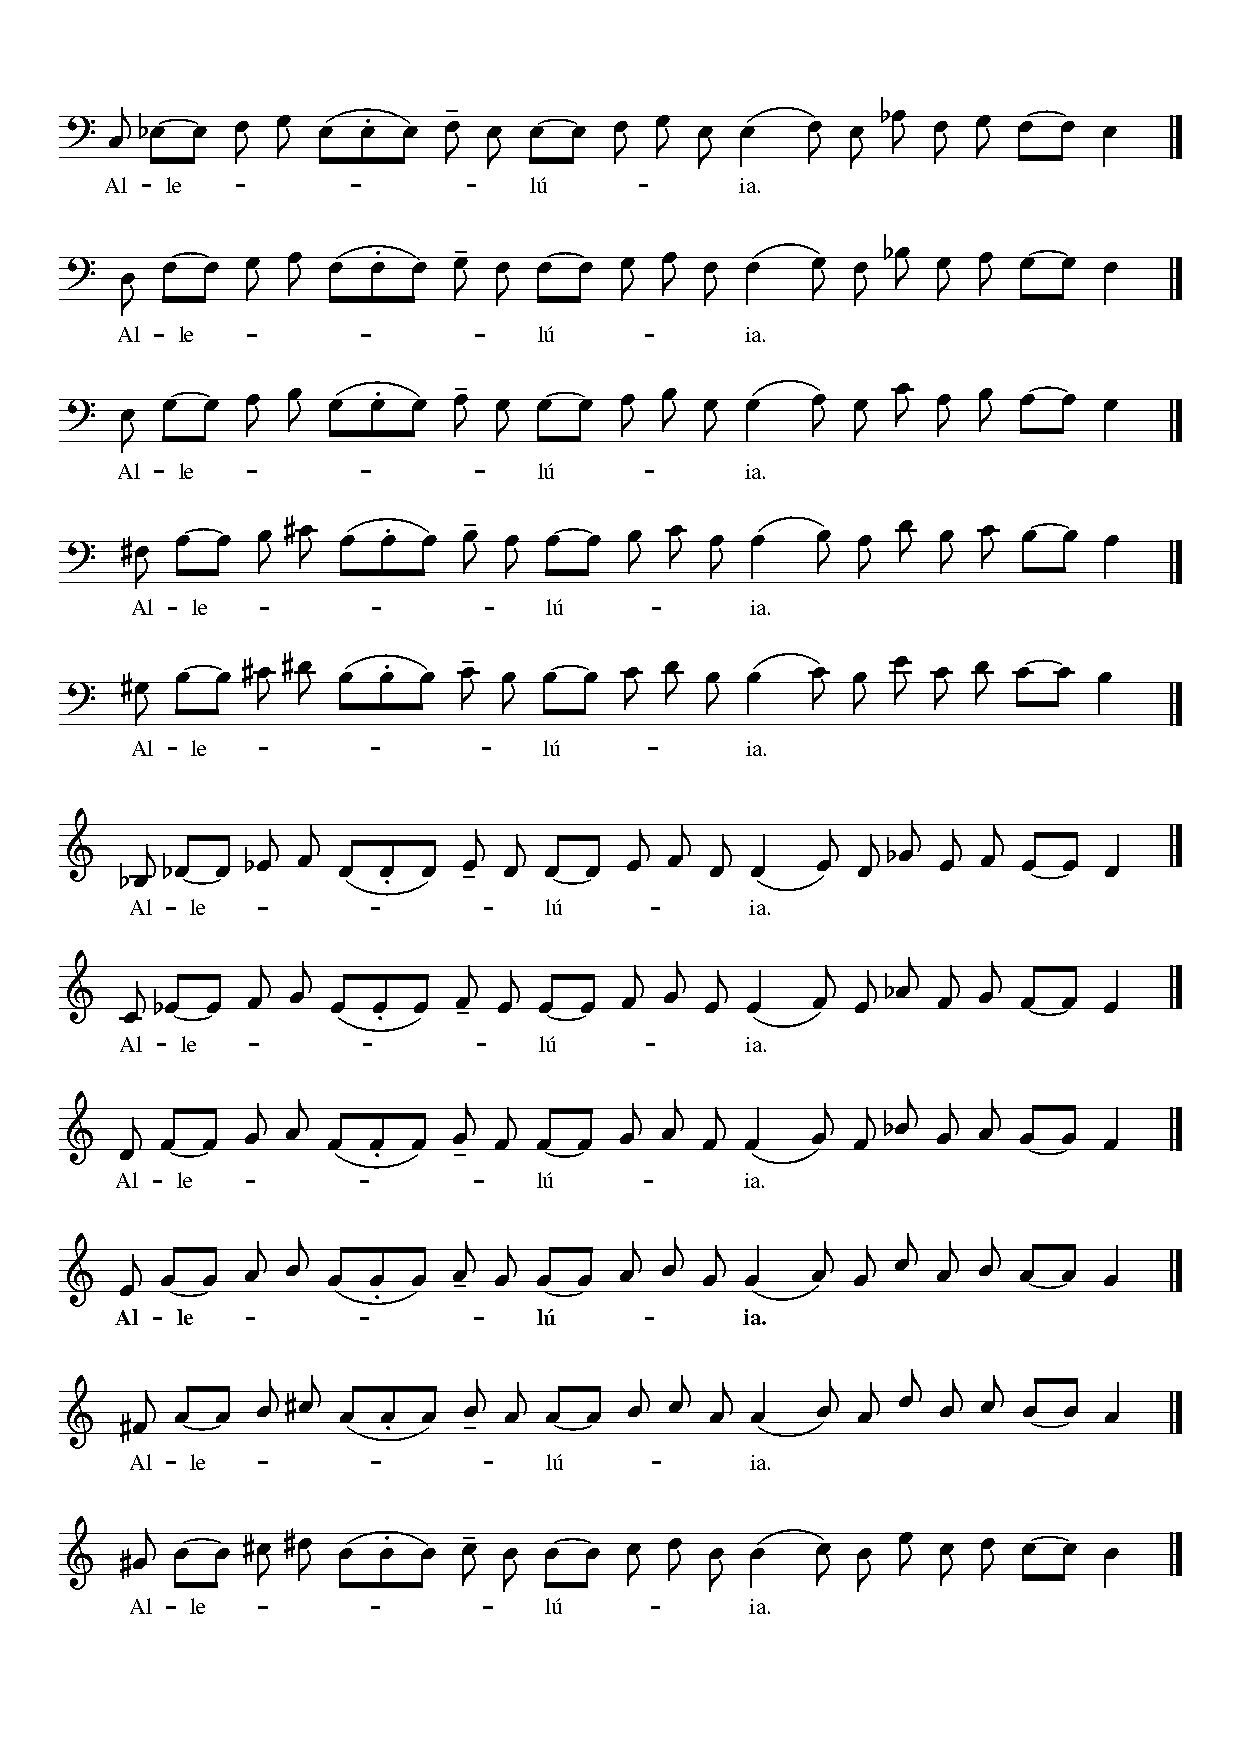
\includepdf[pages=-]{Alleluia_transpozycje.pdf}
\end{document}
